% -----------------------------*- LaTeX -*------------------------------
\documentclass[11pt]{report}
\usepackage{scribe_ds603}
\usepackage{tikz}
\usetikzlibrary{positioning, arrows.meta, shapes.geometric}
\begin{document}

\scribe{Sambhav Jain}		% required
\lecturenumber{11}			% required
\lecturedate{01/10/2025}	% required

\maketitle

% ----------------------------------------------------------------------

\section{What is an Adversarial Example?}

\noindent
The key question in adversarial robustness is: 
\[
\textit{What is a good way for the attacker to perturb samples at test time?}
\]

\subsection*{Concept Overview}
Adversarial examples are perturbed versions of valid inputs that cause a trained model to misclassify them. For instance, consider an input \( x \) that is classified as \emph{unsafe}, and a slightly modified input \( x' \) that is visually similar but is classified as \emph{safe}. The perturbation path from \( x \) to \( x' \) illustrates how small, often imperceptible, changes can fool a model.

\begin{figure}[H]
\centering
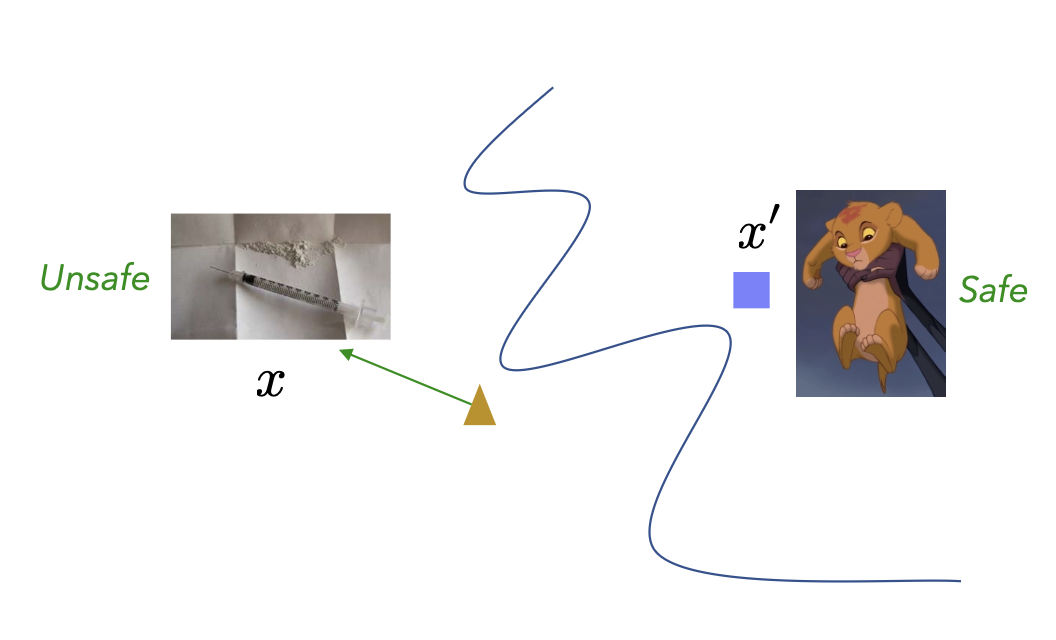
\includegraphics[width=0.7\textwidth]{1.png}
\end{figure}
We have two main kinds of perturbations:\\

\begin{enumerate}[label=(\roman*), leftmargin=*]
\item \textbf{\(\phi\)-divergence perturbations:} These adjust sample probabilities.
    \begin{itemize}
        \item Note: Such perturbations are unlikely to lead to misclassification.
    \end{itemize}

\item \textbf{Optimal transport perturbations:} These lead to strictly stronger attacks than instance-wise perturbations.
\end{enumerate}

\subsection*{Mathematical Formulation}
To understand why, we define:
\[
L_{\epsilon}(\mathcal{H})
:= \mathbb{E}_{\tilde{z} = (\mathbf{x}, y) \sim P^*}
\left[
\sup_{c(\mathbf{x}, \mathbf{x}_{\text{adv}}) \le \epsilon}
\ell\big((\mathbf{x}_{\text{adv}}, y), h\big)
\right].
\]
If we define the Wasserstein ball as:
\[
B_{\epsilon}(P^*)
:= \left\{
Q \,\middle|\,
\inf_{\pi \in \Pi(P^*, Q)}
\int_{\mathbf{x} \times \tilde{\mathbf{x}}}
c(\mathbf{x}, \tilde{\mathbf{x}})\,
d\pi(\mathbf{x}, \tilde{\mathbf{x}})
\le \epsilon
\right\}.
\]
then the following inequality holds:
\[
L_{\epsilon}(\mathcal{H}) \leq \tilde{L}_{\epsilon}(\mathcal{H}),
\]
where
\[
\tilde{L}_{\epsilon}(\mathcal{H}) = \sup_{Q \in B_{\epsilon}(P^*)} \mathbb{E}_{\bar{z} \sim Q} [\ell(\bar{z}, h)].
\]
\textbf{Homework:} Show that the above inequality holds.

\section{Neighborhood-Based Attack}

\textbf{Goal:} Find a perturbation $\delta$ within the neighborhood $N(\cdot)$ such that
\[
h(x + \delta) = \text{Target Incorrect Label}.
\]

\begin{figure}[H]
    \centering
    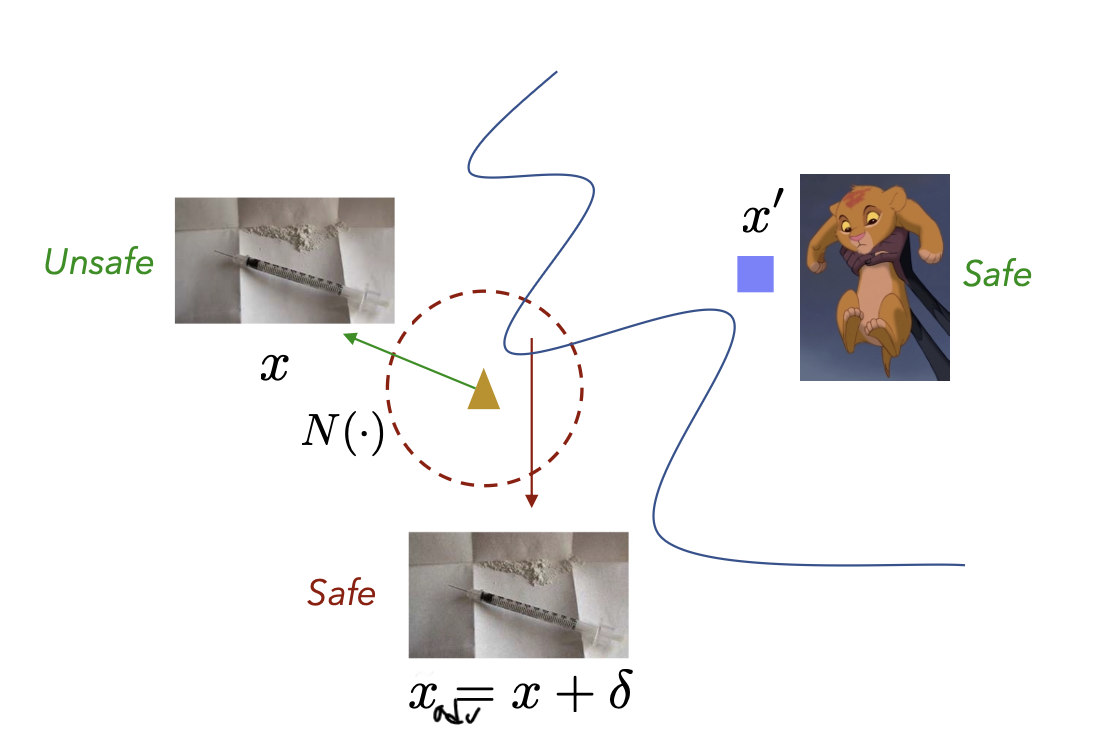
\includegraphics[width=0.6\textwidth]{2.png}
    \caption{Illustration of adversarial perturbation within a neighborhood $N(\cdot)$.
    The attacker searches for $\delta$ within the allowed region so that the model misclassifies $x + \delta$.}
\end{figure}

\noindent
\textbf{Attacker Objective:} Maximize the \emph{Adversarial Loss}.
\[
L_{N}(\mathcal{H})
= \mathbb{E}_{z \sim P^*}
\left[
\sup_{\boldsymbol{x_{\text{adv}}} \in N(\boldsymbol{x})}
\ell\big((\boldsymbol{x_{\text{adv}}}, y), h\big)
\right],
\quad \text{where } z = (\mathbf{x}, y).
\]
\noindent
If the neighborhood $N(\mathbf{x})$ is defined as a norm ball, i.e.
\[
N(\boldsymbol{x}) = \{\, \boldsymbol{x_{\text{adv}}} = \mathbf{x} + \boldsymbol{\delta}
\mid \|\boldsymbol{\delta}\| \le \epsilon \,\},
\]
then the adversarial loss can be written as
\[
L_{N}(\mathcal{H})
= \mathbb{E}_{z \sim P^*}
\left[
\sup_{\|\boldsymbol{\delta}\| \le \epsilon}
\ell\big((\mathbf{x} + \boldsymbol{\delta}, y), h\big)
\right].
\]
\bigskip
\noindent
For \textbf{0-1 Loss} function
\[
L_{N}(\mathcal{H})
= \mathbb{E}_{z \sim P^*}
\left[
\sup_{\mathbf{x}_{\text{adv}} \in N(\mathbf{x})}
\mathbf{1}\big(h(\mathbf{x}_{\text{adv}}) \neq y\big)
\right].
\]
\noindent
\textbf{Attacks in Practice}
\begin{itemize}
    \item \textbf{Neighborhoods:} Typically defined as $\ell_p$-norm balls
    \[
    N(\mathbf{x}) = \{\mathbf{x}_{\text{adv}} = \mathbf{x} + \boldsymbol{\delta} \mid \|\boldsymbol{\delta}\|_p \le \epsilon \},
    \]
    where $\epsilon$ is the perturbation budget.

    \item \textbf{Optimization Formulation:}  
    In practice, the non-differentiable indicator loss $\mathbf{1}(h(\mathbf{x}_{\text{adv}}) \neq y)$  
    is replaced by a smooth proxy loss (e.g., cross-entropy).  
    For a \textbf{\emph{targeted attack}} toward target label $T$, the attacker solves:
    \[
    \min_{\|\boldsymbol{\delta}\| \le \epsilon}
    L_{\text{proxy}}\big((\mathbf{x} + \boldsymbol{\delta}, T), h\big).
    \]

    \item \textbf{Optimization Method:}  
    Typically solved using \emph{Projected Gradient Descent (PGD)} or similar constrained optimization methods.
\end{itemize}
\section{Attacking Linear Classifiers}

For a two-class linear classifier with decision boundary defined by 
\[
\mathbf{w}^\top \mathbf{x} + b = 0,
\]
the predicted label is determined by the sign of \(\mathbf{w}^\top \mathbf{x} + b\). \\
% Place your image right here
\begin{center}
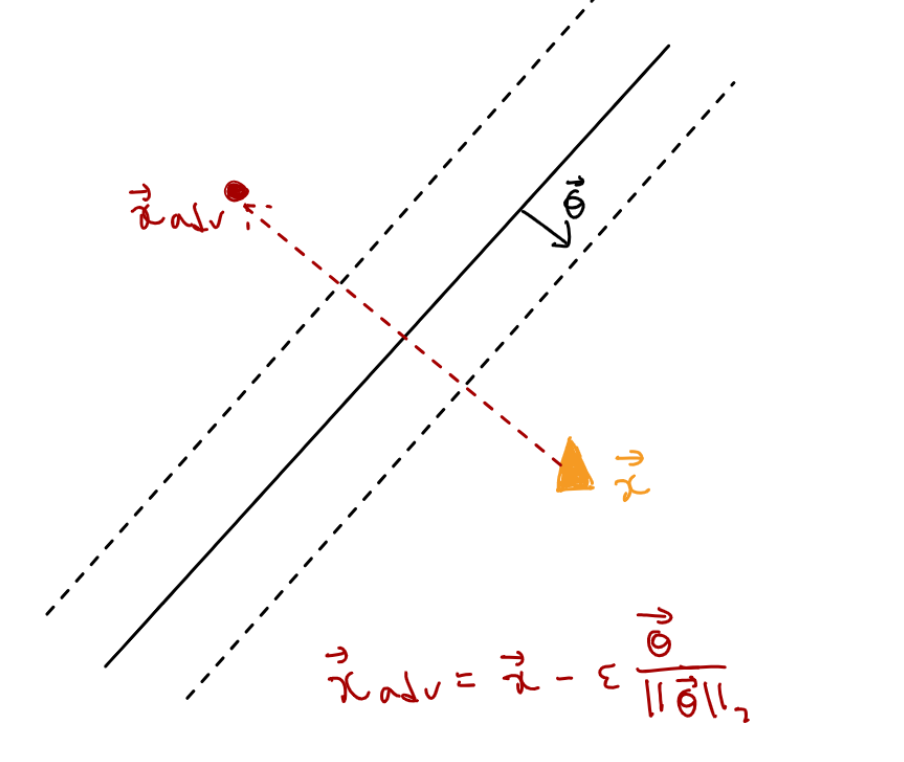
\includegraphics[width=0.4\textwidth]{3.png}
\end{center}

To flip the classification, we want to move the input \(\mathbf{x}\) across the decision boundary with the smallest possible perturbation.  
Since the normal vector to the hyperplane is \(\mathbf{w}\), the most effective direction to change the classifier’s output is \emph{orthogonal to the decision boundary}, i.e., along \(-\mathbf{w}\).
Hence, the adversarial example is chosen as
\[
\mathbf{x}_{\text{adv}} = \mathbf{x} - \epsilon \, \frac{\mathbf{w}}{\|\mathbf{w}\|_2},
\]
where \(\epsilon\) is the \emph{amount of perturbation} or \emph{adversarial budget}.

\bigskip
\section{Overview: Neural Networks}

A feedforward neural network applies a sequence of linear transformations and nonlinear activations to an input 
\begin{center}
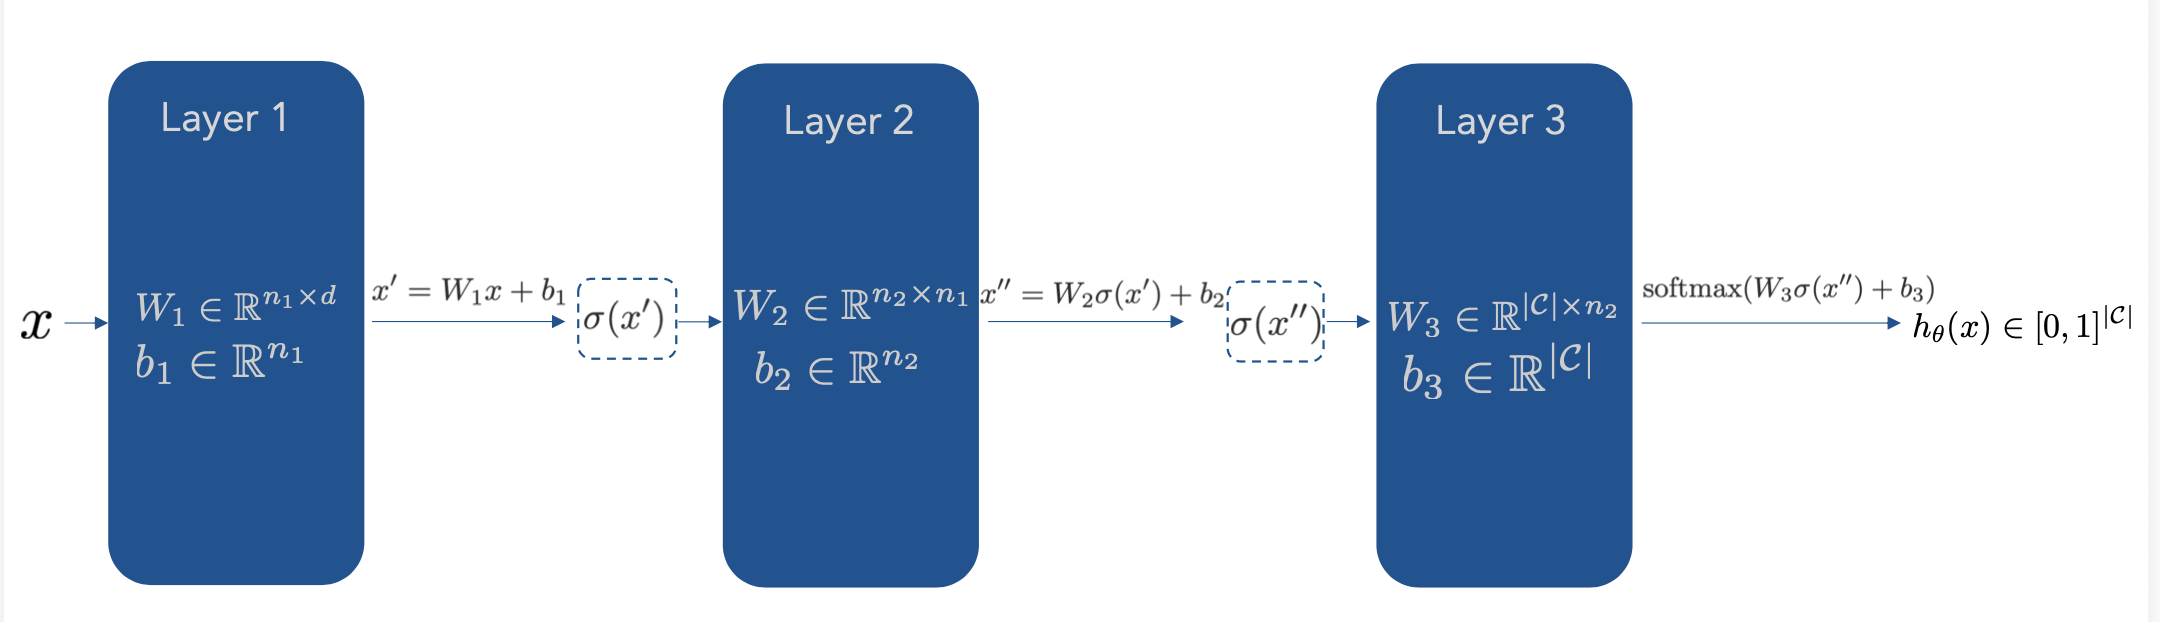
\includegraphics[width=1\textwidth]{4.png}
\end{center}
where $\sigma(\cdot)$ is an element-wise non-linear function (e.g., ReLU)
\[
\sigma(a) =
\begin{cases}
0, & a < 0, \\
a, & a \ge 0,
\end{cases}
\quad
\text{and} \quad
\text{softmax}({a}_i) = \frac{e^{{a}_i}}{\sum_j e^{\tilde{a}_j}}.
\]
and C is the number of classes.

\bigskip
\noindent
The loss is denoted as
\[
\ell((\mathbf{x}, y), h_\theta) = \ell\big((\mathbf{x}, y), h(W_1, b_1, W_2, b_2, W_3, b_3)\big).
\]
\subsection*{Stochastic Gradient Descent}

Each update step to the \textbf{parameters} to minimize the loss is given by:

\[
\boldsymbol{\theta}_{t+1} = \boldsymbol{\theta}_t 
- \eta \, \nabla_{\boldsymbol{\theta}_t} 
\, \ell\big((\vec{x}, y), \boldsymbol{\theta}_t\big)
\]
\begin{center}
where \((\vec{x}, y) \sim \mathcal{D}\)
\end{center}
\smallskip
Here, \(\eta\) is the learning rate that controls the step size,  
and each update is computed using a single (or mini-batch) sample drawn from the data distribution.\\


\section{Single Gradient Ascent Step}
\textbf{Can we use the same idea as SGD to maximize loss over an input?}\\
Yes, Instead of updating model parameters, we perturb the input in the direction that 
\textbf{increases} the loss the most.  
This leads to an \textbf{untargeted adversarial example}:
\[
\vec{x}_{adv} = \vec{x} + \epsilon 
\, \frac{\nabla_{\vec{x}} \ell((\vec{x}, y), h_{\boldsymbol{\theta}})}
{\left\| \nabla_{\vec{x}} \ell((\vec{x}, y), h_{\boldsymbol{\theta}}) \right\|_2}
\]
where $\epsilon$ controls the size of the perturbation, often referred to as the 
\emph{adversarial budget}. \\
Intuitively, this update takes a \textbf{single gradient ascent step} in input space — 
orthogonal to the classifier’s decision boundary — to increase the loss.

\subsubsection*{Why?}

When $\|\boldsymbol{\delta}\|_2 \leq \epsilon$, we can approximate the loss at a perturbed point 
using a first-order Taylor expansion around $\vec{x}$:
\[
\ell(\vec{x} + \boldsymbol{\delta}) 
= \ell(\vec{x}) + \boldsymbol{\delta}^{\top} \nabla_{\vec{x}} \ell(\vec{x}) 
+ \mathcal{O}(\|\boldsymbol{\delta}\|^2)
\]
Ignoring higher-order terms gives:
\[
\ell(\vec{x} + \boldsymbol{\delta}) - \ell(\vec{x}) 
\approx \boldsymbol{\delta}^{\top} \nabla_{\vec{x}} \ell(\vec{x})
\]
Expanding the dot product over dimensions:
\[
\boldsymbol{\delta}^{\top} \nabla_{\vec{x}} \ell(\vec{x}) 
= \sum_{i=1}^{d} \delta_i \, 
\frac{\partial \ell(\vec{x})}{\partial x_i}
\leq \sum_{i=1}^{d} 
|\delta_i| \, 
\left| \frac{\partial \ell(\vec{x})}{\partial x_i} \right|
\]
By the Cauchy–Schwarz inequality:
\[
|\boldsymbol{\delta}^{\top} \nabla_{\vec{x}} \ell(\vec{x})|
\leq \|\boldsymbol{\delta}\|_2 \, 
\|\nabla_{\vec{x}} \ell(\vec{x})\|_2 = \epsilon \, 
\|\nabla_{\vec{x}} \ell(\vec{x})\|_2
\]
The maximum increase occurs when $\boldsymbol{\delta}$ is aligned with the gradient:
\[
\boldsymbol{\delta} = 
\epsilon \, 
\frac{\nabla_{\vec{x}} \ell(\vec{x})}
{\|\nabla_{\vec{x}} \ell(\vec{x})\|_2}
\]
Thus, the adversarial example is:
\[
\vec{x}_{adv} = \vec{x} + \epsilon \, 
\frac{\nabla_{\vec{x}} \ell((\vec{x}, y), h_{\boldsymbol{\theta}})}
{\|\nabla_{\vec{x}} \ell((\vec{x}, y), h_{\boldsymbol{\theta}})\|_2}
\]
Hence, move the input point in the direction of gradient because that \emph{locally increases the loss the most}.

\paragraph{Question:} 
What happens when we constrain $\|\delta\|_\infty \leq \epsilon$ instead? \\ \\
\vspace{0.5em}
To answer this, recall the general inequality:
\[
|\mathbf{a}^\top \mathbf{b}| \leq \|\mathbf{a}\|_p \|\mathbf{b}\|_q, \quad \text{where } \frac{1}{p} + \frac{1}{q} = 1.
\]
This is a generalization of the Cauchy–Schwarz inequality (which corresponds to $p = q = 2$).  \\
For the $\ell_\infty$ constraint, we have $p = \infty$ and $q = 1$, leading to:
\[
\mathbf{a}^\top \mathbf{b} \leq \|\mathbf{a}\|_\infty \|\mathbf{b}\|_1.
\]
Equality holds when $\mathbf{b}$ has the same sign pattern as $\mathbf{a}$~\cite{goodfellow2015explaining}.
Thus, the perturbation that maximizes the loss is aligned with the sign of the gradient:

\[
x_{\text{adv}} = x + \epsilon \, \text{sign}\!\left(\nabla_x \ell((\mathbf{x}, y), h_\theta)\right).
\]
Each input feature is perturbed in the direction of the gradient’s sign.  
Under an $\ell_\infty$ constraint, this causes the largest local increase in loss.

\subsection*{Targeted Adversarial Examples}

\textbf{Q:} How do we move the example such that it is classified in some specific target class $T$?
\vspace{0.5em}\\
In the untargeted setting, we sought perturbations that \emph{maximize} the loss 
$\ell((\mathbf{x}, y), h_\theta)$, making the model more likely to misclassify the input.  
In contrast, a \textbf{targeted} adversarial attack aims to push the input \emph{toward} a chosen target class $T$ by 
\emph{minimizing} the loss $\ell((\mathbf{x}, y_T), h_\theta)$, where $y_T$ is the desired target label.

\[
\mathbf{x}_{\text{adv}} 
= \mathbf{x} - \epsilon \, \frac{\nabla_{\mathbf{x}} \ell((\mathbf{x}, y_T), h_\theta)}
{\|\nabla_{\mathbf{x}} \ell((\mathbf{x}, y_T), h_\theta)\|_p}
\]
This formulation mirrors the untargeted case, except that the gradient direction is reversed, we now move \emph{opposite} to the direction that increases loss for the target label.  

\vspace{0.5em}

\noindent\textbf{Intuition:}  
The targeted perturbation shifts the input so that the model becomes increasingly confident in the chosen target class $T$.  
In geometric terms, the example is moved across the decision boundary and pulled toward the region corresponding to the target class.

\section{White-box Adversarial Examples and Projected Gradient Descent}

In a \textbf{white-box attack}, the adversary has complete access to the model, including its parameters $\theta$, architecture, and gradients. 
This allows direct computation of the loss gradient with respect to the input, $\nabla_x \mathcal{L}(h_\theta(x), y)$, enabling precise perturbations that maximize (or minimize) the loss.
\begin{figure}[H]
    \centering
    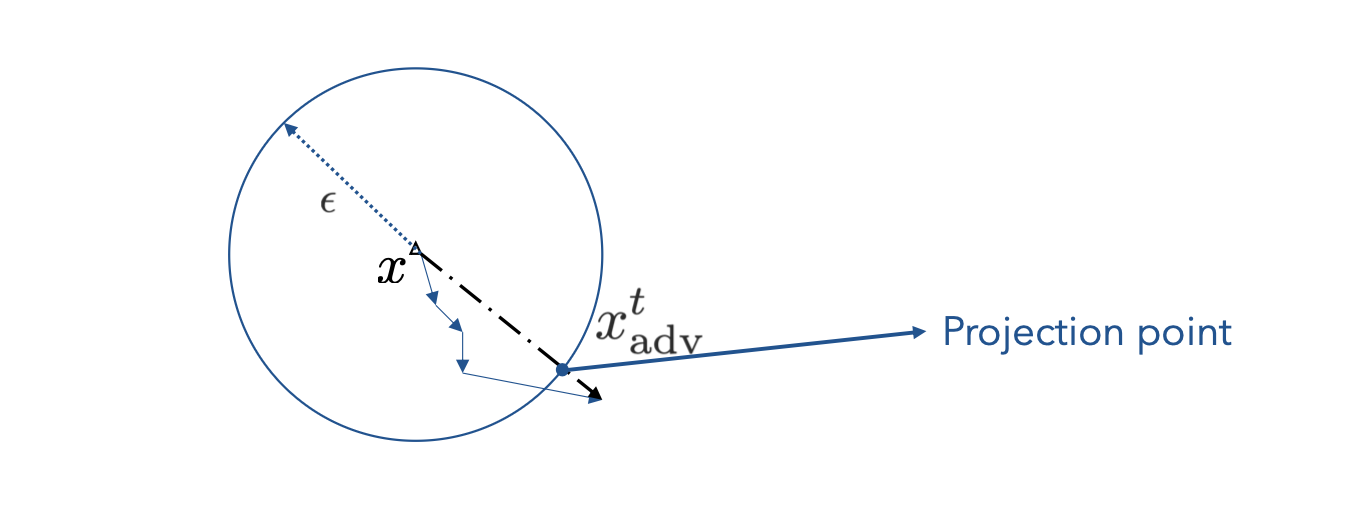
\includegraphics[width=0.6\linewidth]{5.png}
    \caption{White-box adversarial example generation: the adversarial point is iteratively updated and projected back to the $\epsilon$-ball.}
\end{figure}
The iterative update rule for the adversarial example can be written as:
\[
\mathbf{x}_{\text{adv}}^{t} = P_{\mathbf{x}, \epsilon}\left(
\mathbf{x}_{\text{adv}}^{t-1} + 
\alpha \frac{\nabla_{\mathbf{x}_{\text{adv}}^{t-1}} \text{l}((\mathbf{x}_{\text{adv}}^{t-1}, y), h_{\boldsymbol{\theta}})}
{\|\nabla_{\mathbf{x}_{\text{adv}}^{t-1}} \text{l}((\mathbf{x}_{\text{adv}}^{t-1}, y), h_{\boldsymbol{\theta}}||_2}
\right)
\]
where $P_{\mathbf{x}, \epsilon}$ projects the adversarial example back onto an $\epsilon$-ball around the original input $\mathbf{x}$.\\ \\
\textbf{Intuition:} Search iteratively for the empirically strongest perturbation by taking many small gradient steps and projecting back into the allowed \(\epsilon\)-ball.
\vspace{0.5em}
\section{Universal Adversarial Perturbations\cite{moosavi2019universal}}
\textbf{Key Question:} What if we want a single adversarial perturbation that works for multiple different inputs? \\ \\
\begin{figure}[H]
    \centering
    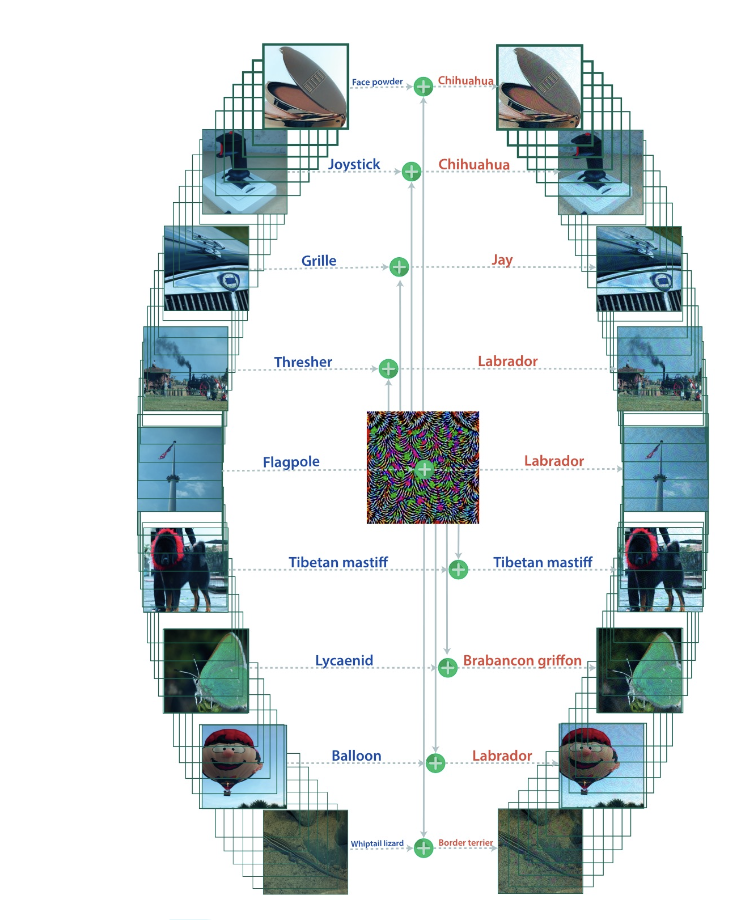
\includegraphics[width=0.6\linewidth]{6.png}
\end{figure}
The Universal Adversarial Perturbation (UAP) algorithm seeks a single, image-agnostic perturbation 
that can fool a classifier across many inputs. It iteratively updates a universal perturbation 
vector $\boldsymbol{\delta}$ by accumulating minimal input-specific perturbations $\mathbf{v}_i$ that cause 
misclassification. After each update, $\boldsymbol{\delta}$ is projected back onto the allowed 
$\ell_p$-ball to keep the perturbation imperceptible, resulting in a universal perturbation that 
generalizes across samples.
\begin{algorithm}[H]
\begin{algorithmic}[1]
\STATE Initialize $\boldsymbol{\delta}^{(0)} = \mathbf{0}$
\FOR{each input $\mathbf{x}_i$}
    \IF{$h_\theta(\mathbf{x}_i + \boldsymbol{\delta}^{(n)}) = h_\theta(\mathbf{x}_i)$}
        \STATE $\mathbf{v}_i \gets \arg\min_{\|\mathbf{r}\|_2 \le \xi} \; h_\theta(\mathbf{x}_i + \boldsymbol{\delta}^{(n)} + \mathbf{r}) \ne h_\theta(\mathbf{x}_i)$
        \STATE $\boldsymbol{\delta}^{(n+1)} \gets P_{\mathbf{x}, \epsilon}\left(\boldsymbol{\delta}^{(n)} + \mathbf{v}_i\right)$
    \ENDIF
\ENDFOR
\end{algorithmic}
\end{algorithm}
\section{Types of Adversarial Attacks}

Below are common categories of adversarial attacks (brief descriptions):

\begin{enumerate}
  \item \textbf{Neighborhood / norm-bounded attacks} \\
  Perturbations constrained to a small neighborhood around the input, e.g.
  \[
    \mathbf{x}_{\text{adv}} = \mathbf{x} + \boldsymbol{\delta}, \qquad \|\boldsymbol{\delta}\|_p \le \epsilon.
  \]

  \item \textbf{Minimum-norm (optimization) attacks} \\
  Find the smallest perturbation that causes misclassification:
  \[
    \min_{\boldsymbol{\delta}} \ \|\boldsymbol{\delta}\|_2 \quad\text{s.t.}\quad h_\theta(\mathbf{x}+\boldsymbol{\delta}) \ne y.
  \]
  These attacks (e.g. Carlini–Wagner) seek perceptually minimal changes that flip the label.

  \item \textbf{Patch-based attacks
} \\
  Localized (often visible) perturbations restricted to a region or patch \(M\):
  \[
    \mathbf{x}_{\text{adv}} = \mathbf{x} + \boldsymbol{\delta}, \qquad \operatorname{supp}(\boldsymbol{\delta}) \subseteq M(\mathbf{x}),
  \]
  where \(\boldsymbol{\delta}\) is nonzero only on a patch (e.g. stickers, adversarial patches) and \(M(\mathbf{x})\) denotes the allowed patch mask/placement.

  \begin{figure}[H]
    \centering
    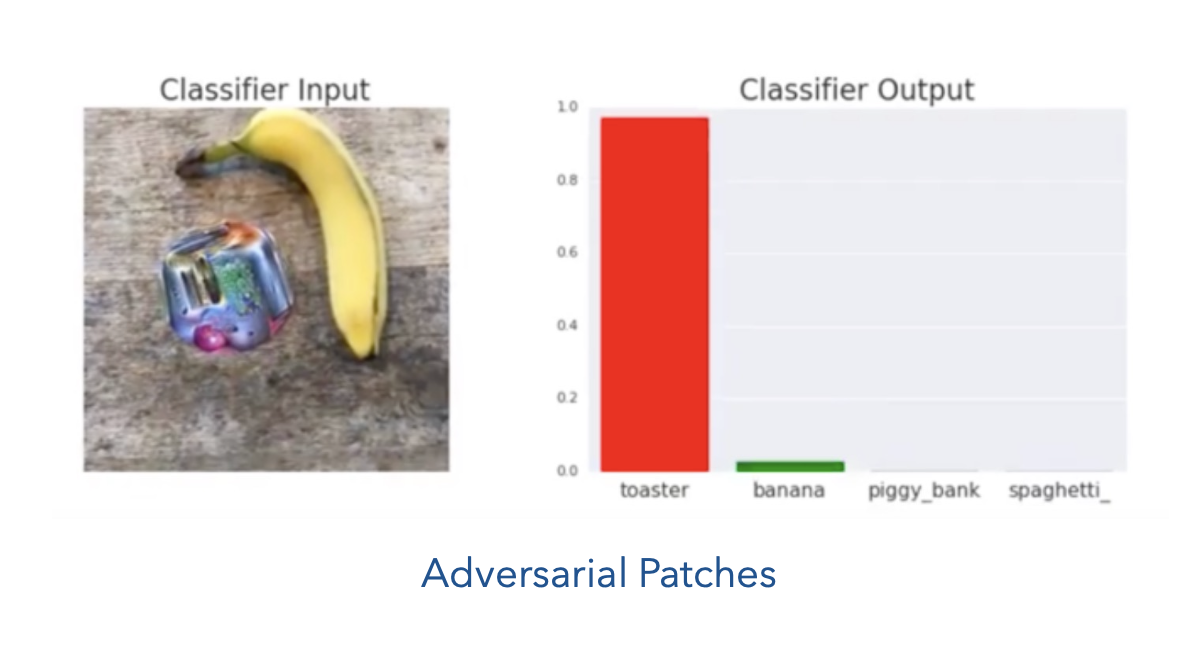
\includegraphics[width=0.6\linewidth]{7.png}
\end{figure}

  \item \textbf{Black-box / query-based attacks} \\
  The adversary does not have access to model internals; attacks rely on queries:
  \begin{itemize}
    \item \emph{Score-based} (or confidence-based): attacker queries the model and uses returned scores/probabilities to estimate gradients or perform optimization.
    \item \emph{Decision-based}: attacker only observes final labels (top-1); algorithms perform boundary-search or estimate minimal perturbations via queries.
  \end{itemize}
  Black-box methods include transfer-based attacks (craft on surrogate models) and iterative query strategies \cite{mao2022adversarial}
.
\end{enumerate}
\begin{figure}[H]
    \centering
    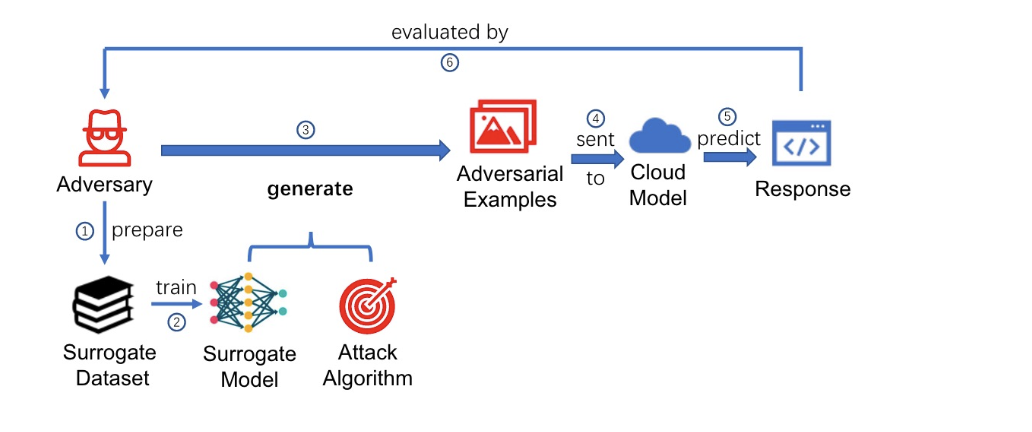
\includegraphics[width=1.0\linewidth]{8.png}
\end{figure}
\bibliographystyle{plain}
\bibliography{refs}
\end{document}
